\documentclass[../main.tex]{subfiles} % required, if the Chapter be a seperate doc

\begin{document}

\chapter{Zusammenfassende Tabellen}\label{ch:zusammenfassende-tabellen}

        \section{Feder 1}\label{sec:feder-1}
    \begin{figure}[H]
        \centering
        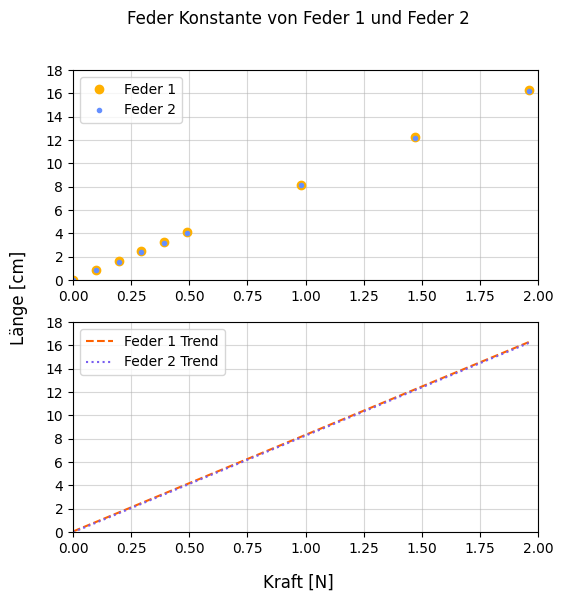
\includegraphics[scale=0.8]{graph/Spring-1-and-Spring-2}
        \caption{Die Darstellung der beiden gemessenen Federn übereinander gesetzt mit Datenpunkte und Trendlinie}
        \label{fig:graph-single-spring-comparisons}
    \end{figure}
    \begin{figure}[H]
        \centering
        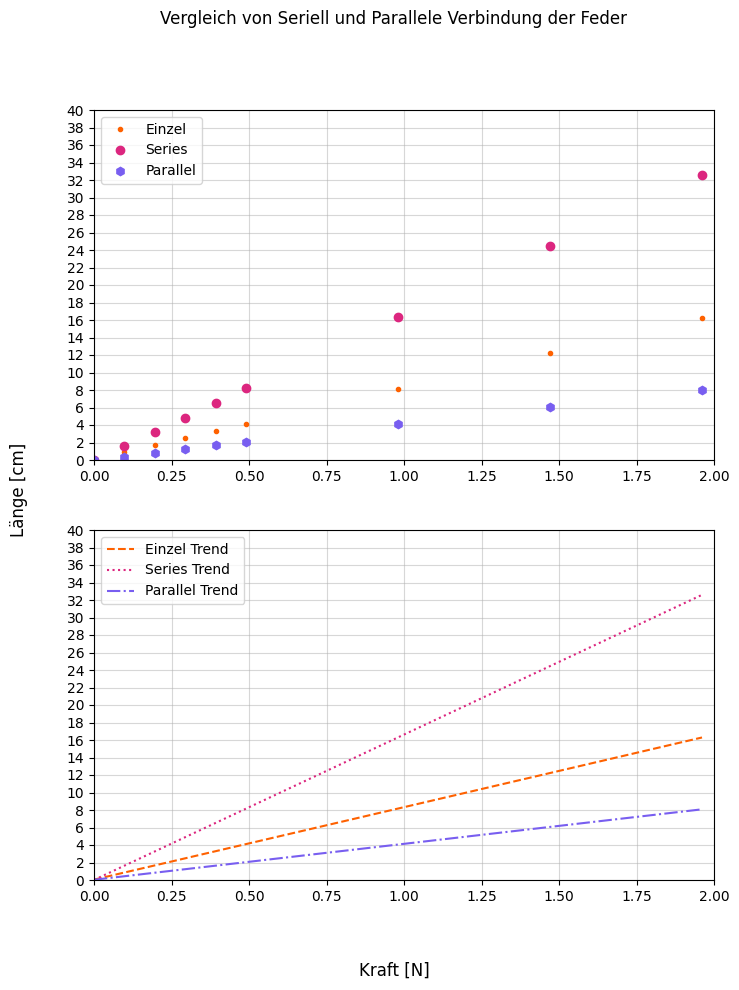
\includegraphics[scale=0.7]{graph/Spring-setup-comparison}
        \caption{Die Darstellung der Feder Positionen einzeln, in Seriell und in Parallel mit Datenpunkte und Trendlinien}
        \label{fig:graph-spring-setup-comparisons}
    \end{figure}
    \section{Arbeit}\label{sec:arbeit}

\end{document}